\documentclass[10pt,a4paper]{article}
\usepackage[utf8]{inputenc}
\usepackage[spanish]{babel}
\usepackage[margin=0.7in]{geometry}
\usepackage{amsmath}
\usepackage{amsfonts}
\usepackage{amssymb}
\usepackage{enumitem}
\usepackage{hyperref} 
\usepackage{graphicx}
\usepackage{url}
\usepackage{array}
\newcolumntype{P}[1]{>{\centering\arraybackslash}p{#1}}
\usepackage{longtable}
\usepackage{breakurl}
\hypersetup{pdftex,colorlinks=true,allcolors=black}
\hypersetup{
    pdftitle={},
    pdfauthor={Pablo Riutort Grande},
    pdfsubject={},
    bookmarksnumbered=true,     
    bookmarksopen=true,         
    bookmarksopenlevel=1,       
    colorlinks=true,            
    pdfstartview=Fit,           
    pdfpagemode=UseOutlines,    % this is the option you were lookin for
    pdfpagelayout=TwoPageRight
}
\usepackage{fancyhdr}
\pagestyle{fancy}
\fancyhf{}
\fancyfoot[C]{\iffloatpage{}{\thepage}}
\renewcommand{\headrulewidth}{0pt}
\renewcommand{\footrulewidth}{0pt}
\usepackage{listings}
\usepackage{xcolor}
\usepackage{hypcap}
\definecolor{codegreen}{rgb}{0,0.6,0}
\definecolor{codegray}{rgb}{0.5,0.5,0.5}
\definecolor{codepurple}{rgb}{0.58,0,0.82}
\definecolor{backcolour}{rgb}{0.95,0.95,0.92}
\lstdefinestyle{mystyle}{
    backgroundcolor=\color{backcolour},   
    commentstyle=\color{codegreen},
    keywordstyle=\color{magenta},
    numberstyle=\tiny\color{codegray},
    stringstyle=\color{codepurple},
    basicstyle=\ttfamily\footnotesize,
    breakatwhitespace=false,         
    breaklines=true,                 
    captionpos=b,                    
    keepspaces=true,                 
    numbers=left,                    
    numbersep=5pt,                  
    showspaces=false,                
    showstringspaces=false,
    showtabs=false,                  
    tabsize=2
}
\lstset{style=mystyle}
\usepackage{xparse}
\NewDocumentCommand{\codeword}{v}{%
\texttt{{#1}}
}
\author{Pablo Riutort Grande}
\title{PEC 3\\ \vspace{1cm}\textbf{Análisis de puertos, vulnerabilidades y protocolos}}
\begin{document}

\maketitle

\section*{Linux Server}
\begin{enumerate}[label=\textbf{\alph*)}]
\item Para instalar Snort se han seguido las instrucciones de la página oficial de Snort \cite{snort}.\\
Primero se instalaron algunas dependencias necesarias \cite{upcloud}:
\begin{lstlisting}[language=bash]
apt-get install -y gcc make libpcre3-dev zlib1g-dev libluajit-5.1-dev libpcap-dev openssl libssl-dev libnghttp2-dev libdumbnet-dev bison flex libdnet
\end{lstlisting}

La instalación consiste en primero instalar DAQ (Data Acquisition library):
\begin{lstlisting}[language=bash]
wget https://www.snort.org/downloads/snort/daq-2.0.7.tar.gz
tar xvzf daq-2.0.7.tar.gz
cd daq-2.0.7
./configure && make && sudo make install
\end{lstlisting}

Durante la instalación hubo algunos problemas de compilación que se solventaron mediante autoreconf
\begin{lstlisting}[language=bash]
autoreconf -f -i; ./configure && make && sudo make install
\end{lstlisting}

Posteriormente podemos instalar Snort:
\begin{lstlisting}[language=bash]
tar xvzf snort-2.9.16.tar.gz
                      
cd snort-2.9.16
./configure --enable-sourcefire && make && sudo make install
\end{lstlisting}

Finalmente, pasamos a ejecutar el comando ldconfig que crea los links necesarios y cachea las diferentes librerías que utilizará Snort \cite{ldconfig}.
\begin{lstlisting}[language=bash]
ldconfig
\end{lstlisting}
\begin{figure}[h!]
  \centering
  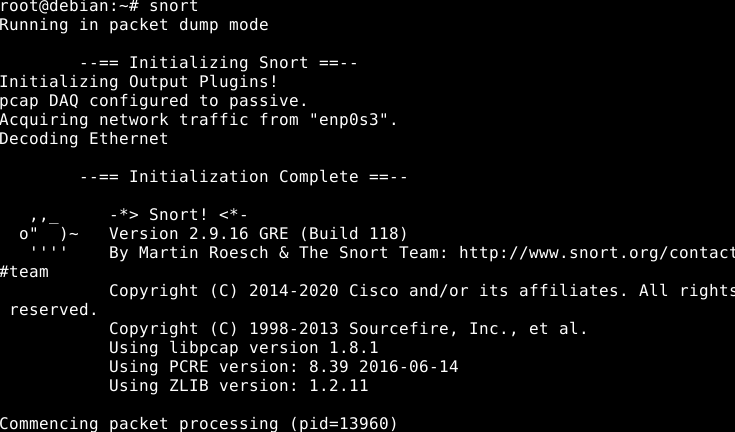
\includegraphics[scale=0.3]{snort.png}\\
  \caption{Snort instalado en el sistema Debian}
  \label{fig:snort}
\end{figure}
\item Para este apartado primero primero tendremos que configurar Snort para funcionar como un NIST (Network Intrusion Detection System). Este modo requiere de tener una estructura de ficheros donde guardar las reglas de Snort y los logs:
\begin{lstlisting}[language=bash]
mkdir -p /etc/snort/rules
chmod -R 5775 /etc/snort
mkdir /var/log/snort
chmod -R 5775 /var/log/snort
mkdir /usr/local/lib/snort_dynamicrules
chmod -R 5775 /usr/local/lib/snort_dynamicrules
\end{lstlisting}
Movemos la configuración de Snort a los nuevos ficheros:
\begin{lstlisting}[language=bash]
mkdir -p /etc/snort/rules
chmod -R 5775 /etc/snort
mkdir /var/log/snort
chmod -R 5775 /var/log/snort
mkdir /usr/local/lib/snort_dynamicrules
chmod -R 5775 /usr/local/lib/snort_dynamicrules
\end{lstlisting}

Creamos los ficheros que contengan las reglas que Snort utilizará para detectar los paquetes:
\begin{lstlisting}[language=bash]
touch /etc/snort/rules/white_list.rules
touch /etc/snort/rules/black_list.rules
touch /etc/snort/rules/local.rules
\end{lstlisting}
Editamos local.rules:
\begin{lstlisting}[language=bash]
alert icmp any any -> $HOME_NET any (msg:"uoc - ping"; itype: 8; sid:1; rev:1;)
\end{lstlisting}
Esta regla indica que cualquier paquete ICMP de cualquier origen y cualquier puerto dirigido a la red local y a cualquier puerto será registrado como "uoc - ping". Además, se le añade la opción de que itype sea 8 para que detecte los paquetes echo request del protocolo ICMP (ping) \cite{icmp8}

\begin{lstlisting}[language=c, caption={Extracto de src/decode.h de Snort donde se incluyen los distintos tipos de ICMP}]
#define ICMP_ECHO               8    /* Echo Request                 */
\end{lstlisting}

Para utilizar estas reglas debemos editar el fichero de configuración en /etc/snort/snort.conf indicando el path correcto de las reglas de Snort y comentar aquellas que no tengamos pero que Snort espera encontrar:
\begin{lstlisting}[language=bash, caption={Los path de los rules quedan ahora bajo /etc/snort/}]
var RULE_PATH rules
var SO_RULE_PATH so_rules
var PREPROC_RULE_PATH preproc_rules
\end{lstlisting}

\begin{lstlisting}[language=bash, caption={Quedan deshabilitadas las reglas a excepción de local.rules}]
# site specific rules
include $RULE_PATH/local.rules

#include $RULE_PATH/app-detect.rules
#include $RULE_PATH/attack-responses.rules
...
\end{lstlisting}

Podemos validar la configuración mediante:
\begin{lstlisting}[language=bash]
snort -T -c /etc/snort/snort.conf
\end{lstlisting}

Finalmente podemos ejecutar Snort en modo NIST aplicando las reglas y la configuración mediante el comando:
\begin{lstlisting}[language=bash]
snort -A console -i enp0s3 -c /etc/snort/snort.conf
\end{lstlisting}

\begin{figure}[h!]
  \centering
  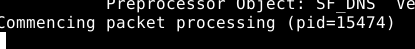
\includegraphics[scale=0.6]{snort2.png}\\
  \caption{Snort empieza a escuchar conexiones}
  \label{fig:snort2}
\end{figure}

\begin{figure}[h!]
  \centering
  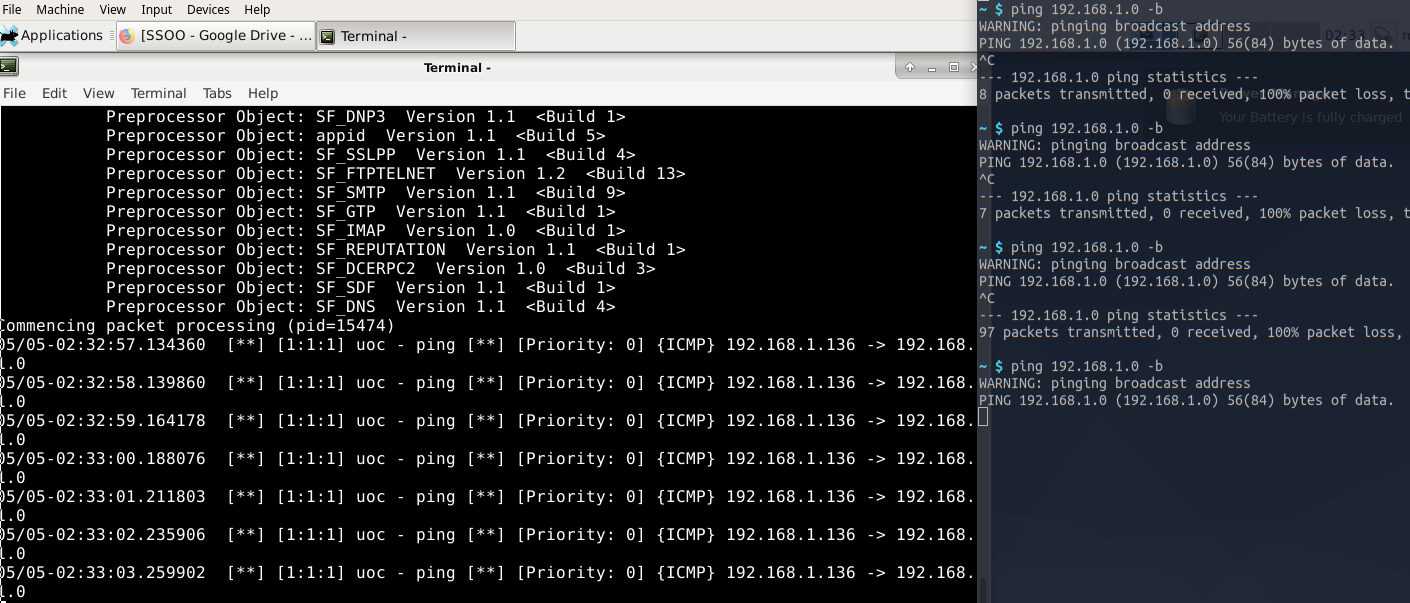
\includegraphics[scale=0.3]{snort3.png}\\
  \caption{Lanzamos ping desde la máquina local y es detectado por Snort}
  \label{fig:snort2}
\end{figure}

\item El servicio SSH ya quedó instalado para la PEC anterior, para configurarlo podemos editar el archivo /etc/ssh/sshd\_config mediante el editor de vim. Para este ejercicio se realizarán prácticamente las mismas acciones con vim sobre distintas líneas del archivo sshd\_config:
\begin{enumerate}[label=\arabic*.]
\item Buscar el contenido correspondiente a la acción a ejecutar con el comando ``/$<$palabra(s) a buscar$>$''
\item Descomentar la línea si está comentada borrando el carácter ``\#'' del inicio de línea con el comando ``x''.
\item Cambiar el parámetro situándonos sobre él mediante el comando ``w'', editándolo mediante ``cw'' y escribiendo el contenido deseado.
\item Guardamos el contenido del archivo pasando a modo normal (Esc.) y escribiendo el comando ``:w''.
\item Después de cada edición será necesario reiniciar el servicio mediante el comando ``systemctl ssh restart''.
\end{enumerate}
\begin{itemize}

\item Para cambiar el puerto para que el servicio se ejecute en el puerto 3333 esta acción buscamos el puerto 22 con el comando de búsqueda ``/Port 22''. Lo descomentamos borrando el carácter ``\#'' del inicio y cambiamos el número 22 por el 3333:

\begin{figure}[h!]
  \centering
  
\includegraphics[scale=0.6]{ssh1.png}\\
  \caption{Edición del archivo sshd\_config para configurar el puerto 3333}
  \label{fig:port22}
\end{figure}

\item Para evitar que el root se conecte de forma remota podemos editar la línea del archivo donde pone PermitRootLogin a PermitRootLogin No.

\begin{figure}[h!]
  \centering
  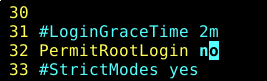
\includegraphics[scale=0.6]{ssh2.png}\\
  \caption{Edición del archivo sshd\_config para restringir el acceso root}
  \label{fig:loginno}
\end{figure}
\pagebreak

\item Para limitar el número máximo de intentos a 3 podemos cambiar la línea donde pone MaxAuthTries a MaxAuthTries 3.

\begin{figure}[h!]
  \centering
  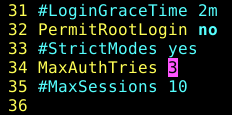
\includegraphics[scale=0.6]{ssh3.png}\\
  \caption{Edición del archivo sshd\_config para configurar el máximo número de intentos de autenticación a 3}
  \label{fig:tries}
\end{figure}

\item Para limitar el tiempo máximo de login a 60 segundos podemos editar la línea donde pone LoginGraceTime a LoginGraceTime 1m. Si pasado el tiempo límite se introduce una contraseña, el sistema cierra la conexión y muestra el mensaje: ``Connection closed by 192.168.1.199 port 3333''

\begin{figure}[h!]
  \centering
  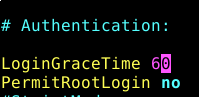
\includegraphics[scale=0.6]{ssh4.png}
    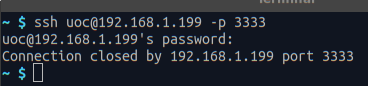
\includegraphics[scale=0.6]{ssh5.png}\\
  \caption{Edición del archivo sshd\_config para limitar el tiempo que se permite para hacer login y una muestra del mensaje recibido por parte de la máquina virtual en caso de exceder dicho tiempo.}
  \label{fig:loggintime}
\end{figure}

\item Para impedir el login mediante de password se puede editar la línea que contiene PasswordAuthentication por PasswordAuthentication no
\begin{figure}[h!]
  \centering
  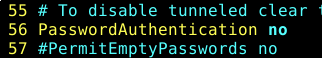
\includegraphics[scale=0.6]{ssh6.png}\\
  \caption{Edición del archivo sshd\_config para restringir el acceso por password}
  \label{fig:passauth}
\end{figure}

\item Para configurar el uso de clave pública-privada para poder acceder al servidor primero generamos una clave SSH en el host \cite{keygen}:
\begin{lstlisting}[language=bash]
ssh-keygen -t rsa -b 4096 -C "pablo.riutort@gmail.com"
\end{lstlisting}
Después de seguir el proceso de generación, este comando generará el directorio .ssh en el directorio del usuario en /home que a su vez contendrá los archivos id\_rsa e id\_rsa.pub que son la clave privada y pública respectivamente.
Para poder copiar la clave SSH pública tenemos que desactivar momentáneamente la restricción de acceso por contraseña y podemos ejecutar el comando \cite{sshcopy}:
\begin{lstlisting}[language=bash]
ssh-copy-id -i .ssh/id_rsa.pub uoc@192.168.1.199 -p 3333
\end{lstlisting}
Que nos copiará la clave SSH del host para acceder únicamente con la clave pública.\\

Ahora, modificamos el archivo de configuración editando la línea que contiene PubkeyAuthentication a PubkeyAuthentication yes y volvemos a aplicar la restricción de PasswordAuthentication del punto anterior y ya podemos acceder sin password únicamente con nuestra clave SSH[\ref{fig:sshcopy}].
\begin{figure}[h!]
  \centering
  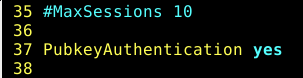
\includegraphics[scale=0.4]{ssh8.png}\\
  \caption{Edición del archivo sshd\_config para configurar el acceso mediante clave pública}
  \label{fig:pubkey}
\end{figure}
\begin{figure}[h!]
  \centering
  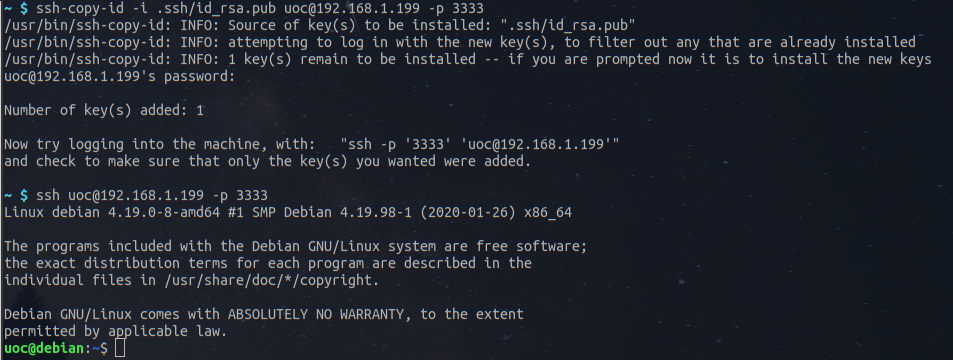
\includegraphics[scale=0.4]{ssh7.png}\\
  \caption{Ejemplo del uso del ssh-copy-id y un acceso con éxito a la máquina virtual mediante ssh sin password}
  \label{fig:sshcopy}
\end{figure}

\end{itemize}


\item Para este ejercicio se ha realizado un escaneo de tipo avanzado mediante la aplicación de Nessus sobre la IP de la máquina virtual de Windows. El programa ha encontrado un total de 49 vulnerabilidades, 12 de las cuales son de riesgo medio, 1 de riesgo alto y 2 de riesgo crítico y las restantes son de carácter informativo.
En la tabla adjunta [Cuadro \ref{table:nessus}] se comentan algunas de las vulnerabilidades encontradas, sus posibles exploits y soluciones.\\

\begin{longtable}{| p{.20\textwidth} | p{.20\textwidth} | p{.20\textwidth} | p{.20\textwidth} |} 
\hline 
 \textbf{Riesgo de seguridad} & \textbf{Descripción} & \textbf{Exploits} & \textbf{Solución} \\ 
\hline 
\multicolumn{4}{|c|}{\textbf{Nivel crítico}} \\ 
\hline 
\textit{KB4025339: Windows 10 Version 1607 Cumulative Update} & Falta la actualización de seguridad KB4025339 & Algunas vulnerabilidades son:
\begin{itemize}
\item Ejecución remota de código
\item Escaladas de privilegios
\item Vulneración de la privacidad de información
\end{itemize}
 & Aplicar la actualización KB4025339\\ 
\hline 
\textit{Mozilla Firefox $<$ 76.0} & La versión de Firefox es anterior a 76.0 & Algunas vulnerabilidades son:
\begin{itemize}
\item Bloqueo de la app potencialmente explotable
\item Desbordamiento de buffer
\item Inyección de comandos
\end{itemize}
 & Actualizar versión de Firefox \\ 
\hline 
\multicolumn{4}{|c|}{\textbf{Nivel alto}} \\ 
\hline 
\textit{Security Updates for Windows Defender (April 2020)} & La versión del motor de Microsoft Windows Defender instalada en el host remoto de Windows es anterior a 4.18.2001.112 & Elevación de privilegios de enlace duro & Habilitar las actualizaciones automáticas para actualizar el motor de escaneo para las aplicaciones antimalware relevantes. \\ 
\hline 
\multicolumn{4}{|c|}{\textbf{Nivel medio}} \\ 
\hline 
 \textit{TLS Version 1.1 Protocol Detection} & El servicio acepta conexión encriptadas con TLS 1.1 y este protocolo no tiene soporte para las soluciones de cifrado actuales y recomendadas 
& 
El uso de versiones antiguas de TLS conlleva ciertos riesgos \cite{bye}, entre ellos:
\begin{itemize}
\item PODDLE\cite{poddle}
\item BEAST\cite{beast}
\item Man-in-the-middle\cite{mitm}
\end{itemize}
& Dar soporte para TLS 1.2 o 1.3 y deshabilitar el 1.1 \\ 
\hline 
\textit{TLS Version 1.0 Protocol Detection} & El servicio acepta conexión encriptadas con TLS 1.0 y este protocolo no tiene soporte para las soluciones de cifrado actuales y recomendadas 
&

\begin{itemize}
\item PODDLE\cite{poddle}
\item BEAST\cite{beast}
\item Man-in-the-middle\cite{mitm}
\end{itemize}
& Dar soporte para TLS 1.2 o 1.3 y deshabilitar el 1.0\\ 
\hline
\textit{SSL Self-Signed Certificate} & La cadena de certificados X.509 para este servicio no está firmada por una autoridad certificadora reconocida. Si el host remoto es un host público en producción, queda anulado el uso de SSL 
& 
\begin{itemize}
\item Man-in-the-middle\cite{mitm}
\end{itemize}
& Comprar o generar un certificado SSL apropiado\\ 
\hline 
\textit{SSL RC4 Cipher Suites Supported} & 
El host remoto admite el uso de cifrado RC4.
El cifrado RC4 es defectuoso a la hora de generar un flujo pseudo aleatorio de bytes introduciendo varios pequeños bias reduciendo así la aleatoriedad. Si un texto es cifrado repetidas veces un atacante podría deducir el texto original. 
& 
\begin{itemize}
\item Bar Mitzvah\cite{bar}
\end{itemize}
& Reconfigurar los servicio para que eviten el uso de RC4. Se recomienda utilizar TLS 1.2 con AES-GCM.\\ 
\hline
\textit{SSL Medium Strength Cipher Suites Supported} & 
El host remoto admite el uso de cifrados SSL de fuerza media (cifrados que usan longitudes de entre 64 y 112 bits).
&
\begin{itemize}
\item SWEET32\cite{sweet32}\cite{tls}
\end{itemize}
& Reconfigurar los servicio para que eviten el uso de RC4. Se recomienda utilizar TLS 1.2 con AES-GCM.\\ 
\hline
\textit{SSL Certificate Wrong Hostname} & El '\textit{commonName}' (CN) del certificado SSL presentado es para una máquina distinta.
&
Tiene varias vulnerabilidades \cite{improper}, entre ellas:
\begin{itemize}
\item Spoof Certificates\cite{spoof}
\item Homograph attack\cite{homo}
\item Man-in-the-middle\cite{mitm}
\end{itemize}
& Comprar o generar un certificado SSL apropiado\\ 
\hline
\textit{SSL Certificate Cannot Be Trusted} & El certificado X.509 del servidor no es de confianza.
& 
\begin{itemize}
\item Man-in-the-middle\cite{mitm}
\end{itemize}
& Comprar o generar un certificado SSL apropiado\\ 
\hline
\textit{Windows Speculative Execution Configuration Check} & El host no ha mitigado adecuadamente una serie de vulnerabilidades de ejecución especulativas conocidas
& 
Algunos exploits son:
\begin{itemize}
\item \textit{Branch Target Injection}
\item \textit{Bounds Check Bypass}
\item \textit{Rogue Data Cache Load}
\end{itemize}
& Aplicar la configuración recomendada por el proveedor.\\ 
\hline
\textit{Security Updates for Windows 10 / Windows Server 2016 (August 2018)} & Al host remoto de Windows le falta una actualización de seguridad. 
& 
Faltan actualizaciones de microcódigo para mitigar vulnerabilidades de hardware conocidos como \textit{Meltdown} y \textit{Spectre} \cite{meltspec}.
& Aplicar las actualizaciones de seguridad de Microsoft para Windows 10.\\ 
\hline
\caption{Vulnerabilidades encontradas por el programa Nessus}
\label{table:nessus}
\end{longtable}

\pagebreak
\item La ejecución de Lynis muestra una serie de componentes analizados divididos en secciones. En cada sección hay una serie de elementos que muestra el objeto a analizar y el resultado obtenido. Por ejemplo, en la sección de SSH el análisis considera que el ClientAliveInterval es aceptable, sin embargo tiene sugerencias para las opciones de AllowTcpForwarding, ClientAliveCountMax, Compression, LogLevel, MaxSessions, TCPKeepAlive, X11Forwarding y AllowAgentForwarding.\\

Los resultados finales de Lynis son 1 advertencia (Warning) sobre el módulo de iptables, que está cargado en el sistema y no tiene reglas activas \href{https://cisofy.com/lynis/controls/FIRE-4512/}{[FIRE-4512]} y 45 sugerencias que paso a resumir a continuación:

\begin{itemize}
\item Se debería considerar el endurecimiento de servicios de sistema.
\item Deshabilitar explícitamente el core dump del archivo /etc/security/limits.conf.
\item Instalar un módulo de PAM para revisar la fuerza de los passwords. Revisar la configuración de PAM.
\item Configurar un algoritmo de encriptación mínimo y máximo en el archivo /etc/login.defs. También propone un tiempo máximo y mínimo para las contraseñas.
\item Añadir fecha de expiración para las cuentas protegidas con contraseña.
\item Deshabilitar módulos del kernel que no se utilizan
\item Deshabilitar los drivers de almacenamiento de USB cuando no se usen
\item Revisar la configuración del DNS
\item Utilizar una herramienta que revise periódicamente las actualizaciones
\item Revisar si una serie de protocolos se utilizan en el sistema
\item Cambiar la configuración de HTTPS y SSL
\item Endurecer la configuración de SSH.
\item Revisar archivos eliminados en uso y su razón
\item Instalar algún software de detección de malware
\end{itemize}


Finalmente, Lynis muestra los detalles del escaneo: \textit{hardening index} de 66, 261 tests realizados y la presencia del componente de Firewall pero también la ausencia de un detector de malware. El escaneo ha sido realizado en modo normal y los módulos eran los de \textit{Security Audit} y \textit{Vulnerability Scan}.

\end{enumerate}

\section*{Windows Server}
\begin{enumerate}[label=\textbf{\alph*)}, start=6]
\item Los sistemas que utilizan NTLM (Windows NT LAN Manager) guardan las credenciales del usuario en memoria y concretamente, guardan un hash del password del usuario que desea autenticarse llamado \textit{NTLM Hash Password}. Esta memoria está gestionada por el proceso \textit{Local Security Auth} o LSASS.EXE. De esta forma, se consigue efectuar el \textit{Single Sign-On} evitando que el usuario deba autenticarse múltiples veces para acceder a recursos de red: Cuando se desea acceder a un recurso se produce un proceso de autenticación entre el recurso, el LSASS y el \textit{Domain Controller}, que guarda el hash NTLM de cada usuario para hacer pruebas de autenticación.\\
El ataque \textit{Pass-the-Hash} o PtH consiste en obtener los credenciales (nombre de usuario y hash NTLM) guardados en memoria por el LSASS y utilizarlos para acceder lateralmente a otros sistemas de la red y hacer escalada de privilegios. No es necesario descifrar el hash para obtener el texto plano, el ataque vulnera el protocolo de autenticaciónan ya que el hash del password permanece estático pero sí que es necesario tener permisos de administrador local para llevarlo a cabo ya que es necesario leer la memoria de LSASS. \cite{PtH}\\
Las buenas prácticas de seguridad son la manera de mitigar el PtH, entre ellas:
\begin{itemize}
\item \textbf{Modelo de seguridad con privilegios mínimos}: Reducir la escalada de privilegios del atacante. El limitar los derechos de administración innecesarios reduce la posibilidad de tener un NTLM hash accesible para un atacante.
\item \textbf{Rotación frecuente de contraseñas}
\item \textbf{Separación de privilegios}: Reducir el alcance de uso de cuentas de administrador separando las cuentas privilegiadas de las no privilegiadas y reducir así el movimiento lateral.
\end{itemize}
Otras maneras de prevenir este tipo de ataques es utilizar herramientas de seguridad como antivirus, firewalls o IDS o configurar el sistema para que no utilice NTLM.\\


Microsoft LAPS (Local Administrator Password Solution) es una herramienta que permite administrar y rotar contraseñas de administrador local \cite{laps} en ordenadores de un mismo dominio de tal forma que estas son únicas en cada ordenador, generadas aleatoriamente y almacenadas de manera segura en la infraestructura del ActiveDirectory y protegidas en el transporte con cifrado del protocolo Kerberos v5, mitigando así la vulnerabilidad de PtH impidiendo el movimiento lateral y la escalada de privilegios \cite{mslaps}. 

Una vez instalado el programa podremos editar los parámetros de las contraseñas como una GPO desde el editor de políticas.

\begin{figure}[h!]
  \centering
  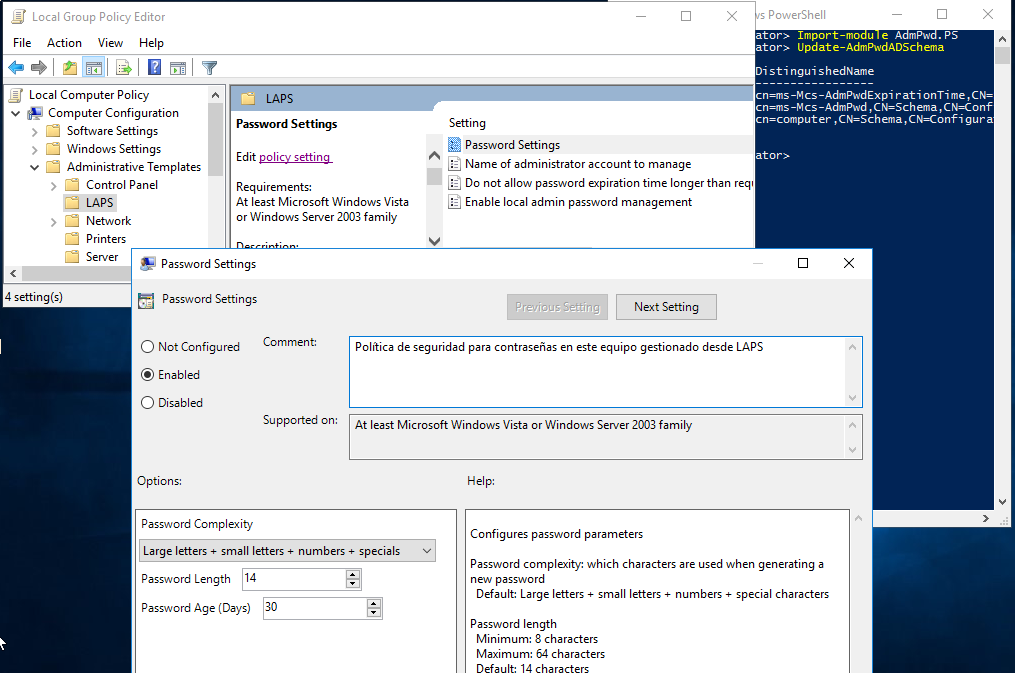
\includegraphics[scale=0.3]{laps.png}\\
  \label{fig:la}
  \caption{Uso de LAPS desde el editor de políticas}
\end{figure}

En la imagen adjunta podemos ver cómo después de habilitar el módulo desde PowerShell (derecha), el módulo de LAPS está disponible como una Local Computer Policy. En el menú de LAPS (izquierda) tendremos varias opciones de las comentadas anteriormente, entre ellas encontramos la primera, Password Settings, que nos permite definir los parámetros de las contraseñas con opciones como la la complejidad, que este contexto son los grupos de caracteres de los que se compone, longitud o la duración de su validez (abajo).\\
Las siguientes configuraciones hacen referencia a la cuenta de administrador sobre la que aplicar estas restricciones, limitar la expiración de la contraseña a lo que dicte esta política y habilitar la delegación de la gestión de la contraseña del administrador local a esta política.

\end{enumerate}

\pagebreak
\begin{thebibliography}{9}

\bibitem{snort}
  Snort,\\
  \textbf{Get started},\\
  \url{https://www.snort.org/#get-started}

\bibitem{upcloud}
  Upcloud,\\
  \textbf{Installing snort on Debian},\\
  \url{https://upcloud.com/community/tutorials/installing-snort-on-debian/}
  
\bibitem{aclocal}
  Stack Overflow,\\
  \textbf{How to overcome “'aclocal-1.15' is missing on your system” warning?},\\
  \footnotesize
  \url{https://stackoverflow.com/questions/33278928/how-to-overcome-aclocal-1-15-is-missing-on-your-system-warning}
  \normalsize

\bibitem{ldconfig}
   ldconfig,\\
   \textbf{ldconfig(8) - Linux man page},\\
   \url{https://linux.die.net/man/8/ldconfig}

\bibitem{icmp8}
	ICMP echo request,\\
	\textbf{Internet Control Message Protocol (ICMP) Parameters - Type 8},\\
	\url{http://www.iana.org/assignments/icmp-parameters/icmp-parameters.xhtml#icmp-parameters-codes-8}

\bibitem{keygen}
	GitHub.com,\\
	\textbf{Generar una nueva clave SSH y agregarla al ssh-agent},\\
	  \footnotesize
	\url{https://help.github.com/es/github/authenticating-to-github/generating-a-new-ssh-key-and-adding-it-to-the-ssh-agent}
	  \normalsize
	  
\bibitem{hard1}
	Nixhat solutions,\\
	\textbf{HARDENING SSH CONFIGURATION},\\
	\url{http://www.nixhat.com/2016/04/hardening-ssh-configuration/}

\bibitem{hard2}
	The geek stuff,\\
	\textbf{7 Default OpenSSH Security Options You Should Change in /etc/ssh/sshd\_config},\\
	\url{https://www.thegeekstuff.com/2011/05/openssh-options/}
	
\bibitem{sshcopy}
	ssh.com,\\
	\textbf{ssh-copy-id},\\
	\url{https://www.ssh.com/ssh/copy-id}

\bibitem{poddle}
	National Vulnerability Database (NIST),\\
	\textbf{CVE-2014-3566 - PODDLE},\\
	\url{https://nvd.nist.gov/vuln/detail/CVE-2014-3566}
	
\bibitem{beast}
	National Vulnerability Database (NIST),\\
	\textbf{CVE-2011-3389 - BEAST},\\
	\url{https://nvd.nist.gov/vuln/detail/CVE-2011-3389}
	
\bibitem{mitm}
	Common Vulnerabilities and Exposures (CVE),\\
	\textbf{CVE-2009-3555 - Man-in-the-middle},\\
	\url{https://cve.mitre.org/cgi-bin/cvename.cgi?name=CAN-2009-3555}

\bibitem{bar}
	National Vulnerability Database (NIST),\\
	\textbf{CVE-2015-2808 - Bar Mitzvah},\\
	\url{https://nvd.nist.gov/vuln/detail/CVE-2015-2808}

\bibitem{sweet32}
	National Vulnerability Database (NIST),\\
	\textbf{CVE-2016-2183 - SWEET32},\\
	\url{https://nvd.nist.gov/vuln/detail/CVE-2016-2183}

\bibitem{spoof}
	Common Vulnerabilities and Exposures (CVE),\\
	\textbf{CVE-2003-0355 - Multiple Web Browsers do not do not validate CN on certificates},\\
	\url{https://cve.mitre.org/cgi-bin/cvename.cgi?name=CVE-2003-0355}

\bibitem{homo}
	threat post,\\
	\textbf{Certificates Spoofing Google, Facebook, GoDaddy Could Trick Mobile Users},\\
	\footnotesize
	\url{https://threatpost.com/certificates-spoofing-google-facebook-godaddy-could-trick-mobile-users/104259/}
	\normalsize
	
\bibitem{tls}
	iweb,\\
	\textbf{SSL/TLS issues - POODLE/BEAST/SWEET32 attacks and the End of SSLv3 + OpenSSL Security Advisory},\\
	\footnotesize
	\url{https://bit.ly/3cwPV7O}
	\normalsize

\bibitem{improper}
	Common Weakness Enumeration (CWE),\\
	\textbf{CWE-297: Improper Validation of Certificate with Host Mismatch},\\
	\url{https://cwe.mitre.org/data/definitions/297.html}

\bibitem{bye}
	PCI Security Standards Council,\\
	\textbf{Are You Ready for 30 June 2018? Saying Goodbye to SSL/early TLS},\\
	\footnotesize
	\url{https://blog.pcisecuritystandards.org/are-you-ready-for-30-june-2018-sayin-goodbye-to-ssl-early-tls}
	\normalsize

\bibitem{PtH}
	Beyond Trust,\\
	\textbf{How do you Prevent Pass-the-Hash Attacks},\\
	\url{https://www.beyondtrust.com/resources/glossary/pass-the-hash-pth-attack}

\bibitem{laps}
	Insider Threat Security Blog,\\
	\textbf{Running laps in the race to security},\\
	\url{https://blog.stealthbits.com/running-laps-in-the-race-to-security/}

\bibitem{mslaps}
	Microsoft Download Center,\\
	\textbf{Protección de dispositivos Windows contra ataques de canal lateral de ejecución especulativa},\\
	\url{https://www.microsoft.com/en-us/download/details.aspx?id=46899}
	
\bibitem{meltspec}
	Windows Support,\\
	\textbf{Protección de dispositivos Windows contra ataques de canal lateral de ejecución especulativa},\\
	\footnotesize
	\url{https://support.microsoft.com/es-es/help/4073757/protect-windows-devices-from-speculative-execution-side-channel-attack}
	\normalsize
	

\end{thebibliography}

\end{document}